
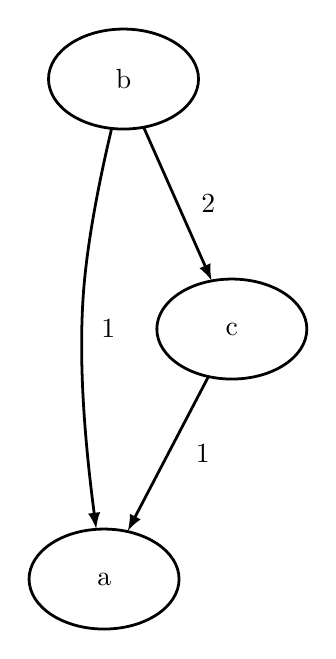
\begin{tikzpicture}[>=latex,line join=bevel,]
  \pgfsetlinewidth{1bp}
%%
\pgfsetcolor{black}
  % Edge: b -> a
  \draw [->] (29.729bp,180.21bp) .. controls (26.323bp,165.91bp) and (21.832bp,144.76bp)  .. (20bp,126bp) .. controls (17.353bp,98.896bp) and (20.017bp,67.83bp)  .. (24.174bp,36.077bp);
  \definecolor{strokecol}{rgb}{0.0,0.0,0.0};
  \pgfsetstrokecolor{strokecol}
  \draw (28.5bp,108bp) node {1};
  % Edge: c -> a
  \draw [->] (64.563bp,90.859bp) .. controls (57.797bp,77.916bp) and (48.175bp,59.508bp)  .. (35.539bp,35.336bp);
  \draw (62.5bp,63bp) node {1};
  % Edge: b -> c
  \draw [->] (41.336bp,180.45bp) .. controls (47.001bp,167.66bp) and (54.947bp,149.74bp)  .. (65.697bp,125.48bp);
  \draw (64.5bp,153bp) node {2};
  % Node: a
\begin{scope}
  \definecolor{strokecol}{rgb}{0.0,0.0,0.0};
  \pgfsetstrokecolor{strokecol}
  \draw (27bp,18bp) ellipse (27bp and 18bp);
  \draw (27bp,18bp) node {a};
\end{scope}
  % Node: c
\begin{scope}
  \definecolor{strokecol}{rgb}{0.0,0.0,0.0};
  \pgfsetstrokecolor{strokecol}
  \draw (73bp,108bp) ellipse (27bp and 18bp);
  \draw (73bp,108bp) node {c};
\end{scope}
  % Node: b
\begin{scope}
  \definecolor{strokecol}{rgb}{0.0,0.0,0.0};
  \pgfsetstrokecolor{strokecol}
  \draw (34bp,198bp) ellipse (27bp and 18bp);
  \draw (34bp,198bp) node {b};
\end{scope}
%
\end{tikzpicture}

